\documentclass[serif,20pt]{beamer}
\usepackage[size=custom,width=90,height=120,orientation=portrait, scale=1.55]{beamerposter}
\useinnertheme{circles}
% \usepackage{mlmodern}
\usepackage{svg}
\usepackage{tikz, pgf}
\usepackage{import}
\usepackage{wallpaper}
\usepackage{csquotes}
\usepackage[super]{natbib}
\usepackage[brazil]{babel}
\usepackage{ragged2e}
\usepackage{caption}
\usepackage{subcaption}
\newcommand{\mathdefault}{}
\settowidth{\leftmargini}{\usebeamertemplate{itemize item}}
\addtolength{\leftmargini}{\labelsep}

\setbeamertemplate{caption}[numbered]

% \usebackgroundtemplate{
\includegraphics[width=\paperwidth,height=\paperheight]{background.png}}

\begin{document}
\begin{frame}[t]
\vspace{5cm}
\begin{columns}
\column{0.2\textwidth}    

\includegraphics[width=\columnwidth]{ppgem.png}
\column{0.6\textwidth}
\begin{center}\Large{%
    \bfseries \MakeUppercase{Redes Neurais Artificiais Integradas para Controle de VANTs}}

    \small{Gabriel D. Silva, Renan S. Geronel, Douglas D. Bueno. Universidade Estadual ``Paulista Júlio de Mesquita Filho'', Câmpus de Ilha Solteira, Engenharia Mecânica, gd.silva@unesp.br, Bolsa de Iniciação Científica --- CNPq}
\end{center}
\column{0.2\textwidth}

\includegraphics[width=\columnwidth]{unesp_logo.png}
\end{columns}

\vspace{5cm}

\begin{columns}[t]
\column{0.45\textwidth}
\begin{block}{\centering\bfseries INTRODUÇÃO}
\vspace{1cm}
\begin{itemize}\justifying
    \item Modelo paramétrico caixa preta.
    \item Determinação das forças de controle a partir da posição inicial e trajetória.
    \item Utilização de redes neurais.
\end{itemize}
\vspace{1cm}
\end{block}
%
\begin{block}{\centering\bfseries OBJETIVO}
\vspace{1cm}
\begin{itemize}\justifying
    \item Desenvolver um algoritmo com redes neurais para controle de forças de de um VANT.
\end{itemize}
\vspace{1cm}
\end{block}
%
\begin{block}{\centering\bfseries MATERIAIS E MÉTODOS}
    \vspace{1cm}
\begin{itemize}\justifying
    \item A determinação das forças de controle será determinada a partir de duas redes neurais.
\end{itemize}
%
\begin{figure}[H]
    \centering
    \caption{Rede Neural}
    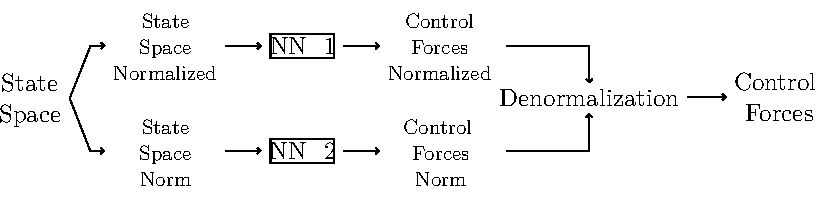
\includegraphics[width=\columnwidth]{../../../report/figures/3methodology/full_scheme.pdf}

    {\footnotesize Fonte: próprio autor.}
    \label{fig:rede_neural}
\end{figure}
\begin{itemize}\justifying
    \item Rede neural é uma técnica de aprendizado de máquina para reconhecimento de padrões.\cite{haykin1999}
\end{itemize}
\begin{figure}
    \centering
    \caption{Rede Neural}
    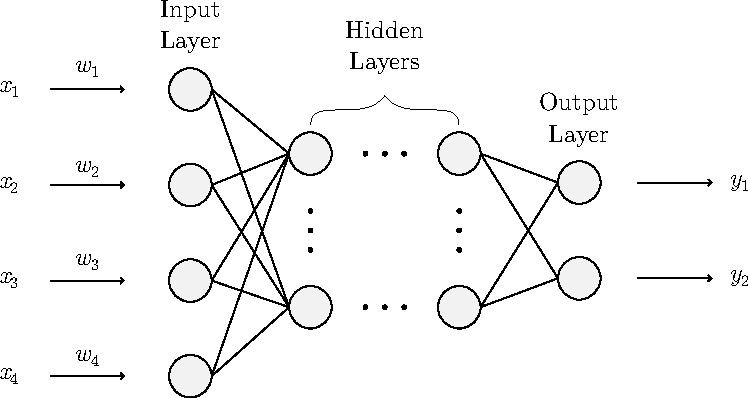
\includegraphics[width=\columnwidth]{../../../report/figures/3review/nn/nn3_ppgem.pdf}
\end{figure}

\begin{itemize}\justifying
    \item Modelo paramétrico de caixa branca para gerar trajetórias.\cite{geronel2023}
    \item As forças de controle são:
    \begin{equation}
        \tau = \begin{bmatrix}
            U_1 & U_2 & U_3 & U_4
        \end{bmatrix}^{\intercal}
    \end{equation}
    \item O vetor de estado é:
    \begin{equation}
        \setcounter{MaxMatrixCols}{20}
        \mathbf{x}_s = \begin{bmatrix}
            x & y & z & \theta & \phi & \psi & \dot{x} & \dot{y} & \dot{z} & \dot{\theta} & \dot{\phi} & \dot{\psi}
        \end{bmatrix}^{\intercal}
    \end{equation}
    \item Uma rede neural do tipo \emph{multi-layer perceptron} foi designada para realizar o treinamento nos dados, em ambas as redes.
\end{itemize}
\vspace{1cm}
\end{block}

\begin{block}{\centering\bfseries RESULTADOS E DISCUSSÕES}
\vspace{1cm}
\begin{itemize}\justifying
    \item A Fig.~\ref{fig:comparison} compara as forças de controle da rede neural em relação às trajetórias do algoritmo do modelo caixa branca.
\end{itemize}
\begin{itemize}
    \item As redes neurais conseguiram reconhecer os padrões.
    \item As forças de controle seguem a tendência das forças reais.
\end{itemize}
\end{block}


\column{0.45\textwidth}

\begin{block}{}

\begin{figure}[H]
    \centering
    \caption{Comparação entre a previsão do modelo e o valor real}
    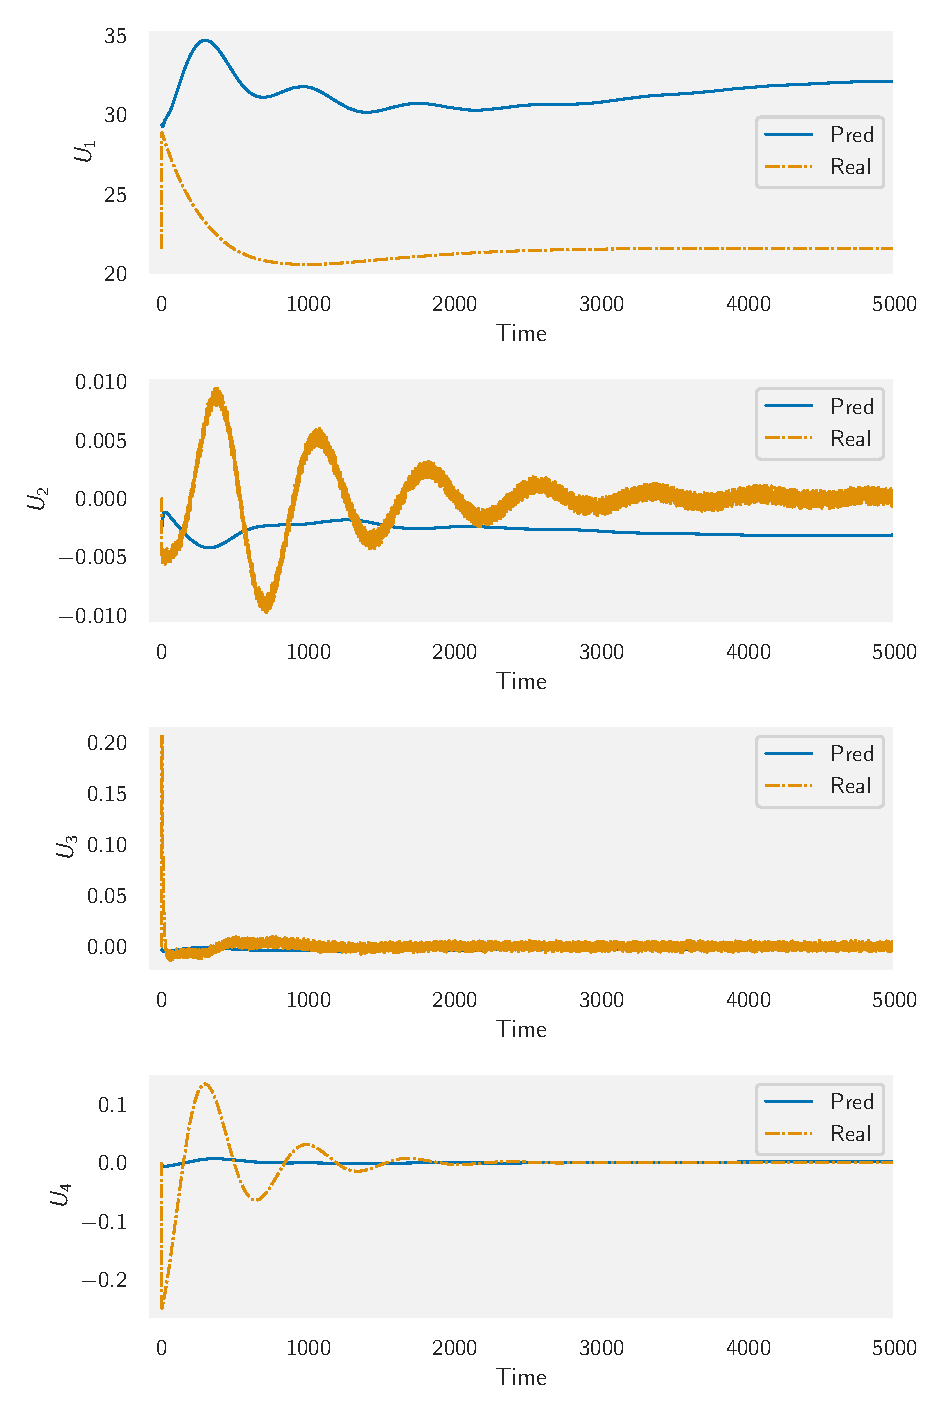
\includegraphics[width=\columnwidth]{../../../report/figures/4results/uav/forces_denormalized.pdf}

    {\footnotesize Fonte: próprio autor.}

    \label{fig:comparison}
\end{figure}
\end{block}

\begin{block}{\centering\bfseries CONCLUSÃO}
\vspace{1cm}
\begin{itemize}\justifying
    \item A rede neural conseguiu determinar as forças de controle de forma satisfatória.
    \item Próximos passos:
    \begin{itemize}\justifying
        \item Simular as trajetórias com os valores obtidos pelo algoritmo.
        \item Sofisticar a rede neural conforme a necessidade.
    \end{itemize}
\end{itemize}
\vspace{1cm}
\end{block}

\begin{block}{\centering\bfseries AGRADECIMENTOS}\justifying
\vspace{1cm}
Os autores agradecem ao Conselho Nacional de Desenvolvimento Científico e Tecnológico (CNPq), proc. no. 406328/2021-8.

\rule{10cm}{0.4pt}

\bibliographystyle{acm}
{\small\bibliography{ref}}
\end{block}


\end{columns}    
\end{frame}
\end{document}